\section{Kinect Hardware}
Microsoft brachte im November 2010 mit dem Produkt Xbox Kinect eine neues Produkt auf den Markt. Mit diesem war es möglich, ihr eigenes Produkt Xbox 360 über eine 3D-Kamera zu steuern und Spiele zu spielen. 
Mit diesem Produkt konnte erstmals ein preiswerter Sensor verwendet werden, um 3D-Bilddaten auszuwerten.
Im Folgenden wird auf die Hardware des Sensors näher eingegangen:

\begin{figure}[H]						
	\centering							
	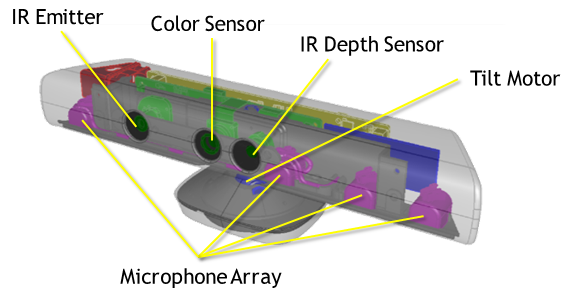
\includegraphics[scale=0.9]{Bilder/kinect_sensor_aufbau.png}			
	\caption{Aufbau Kinect\cite{ws:microsoft_kinect}}						
	\label{f:kinect_hardware}						
\end{figure}



Das Kinectmodul besteht technisch gesehen aus einer RGB Kamera, die maximal eine Auflösung von 1280 x 960 Pixeln unterstützt. 
\cite{webb2012beginning}




\todo{Hardware Bilder}
\todo{erklärungen zu Bilder}
\todo{PrimeSense}
\todo{Triangulation}

Hardware
========

Kippbarer Kopf

Infrarot Projektor

Zwei Kameras

4 Mikrofone -> Für dieses Projekt irrelevant (evtl. Sprachkommandos? Kinect Lib unterstützt Grammatik!!)

Auflösung der Kameras

	color camer 	= max resolution of 1280 x 960 
	depth camera 	= max resolution of 640 x 480.

-Aufbau: 	-Microphonarray zweck=richtung d. Geräusch
			-IR Sensor = Deep Stream
			-RGB Kamera = Bild
-Rauminformationen für Software
-Vorteil: Günstig, leicht zu entwickeln, da SDK vorhanden